\documentclass[conference]{IEEEtran}
\IEEEoverridecommandlockouts
\usepackage{cite}
\usepackage{amsmath,amssymb,amsfonts}
\usepackage{algorithmic}
\usepackage{graphicx}
\usepackage{textcomp}
\usepackage{xcolor}
\usepackage{booktabs}
\usepackage{array}
\usepackage{url}
\usepackage{listings}
\usepackage{multirow}

\lstset{
  basicstyle=\ttfamily\scriptsize,
  breaklines=true,
  frame=single,
  captionpos=b,
  columns=fullflexible,
  keepspaces=true
}

\def\BibTeX{{\rm B\kern-.05em{\sc i\kern-.025em b}\kern-.08em
    T\kern-.1667em\lower.7ex\hbox{E}\kern-.125emX}}

\begin{document}

% ---------------------------------------------------------------
%  TITLE
% ---------------------------------------------------------------
\title{A Multidimensional Data Warehouse and Trend Analytics Framework
for Railway Transit Delay Dynamics: A Case Study of Indian Railways}

% ---------------------------------------------------------------
%  AUTHORS  (fill in your real names / affiliations before submission)
% ---------------------------------------------------------------
\author{
  \IEEEauthorblockN{1\textsuperscript{st} Author Name}
  \IEEEauthorblockA{
    \textit{Dept.\ of Computer Science \& Engineering}\\
    \textit{[University Name]}\\
    City, Country\\
    author1@university.edu}
  \and
  \IEEEauthorblockN{2\textsuperscript{nd} Author Name}
  \IEEEauthorblockA{
    \textit{Dept.\ of Computer Science \& Engineering}\\
    \textit{[University Name]}\\
    City, Country\\
    author2@university.edu}
}

\maketitle

% ---------------------------------------------------------------
%  ABSTRACT
% ---------------------------------------------------------------
\begin{abstract}
India's railway network, one of the largest in the world, generates
billions of operational data points every year, yet much of this
telemetry sits locked in transactional databases never designed for
strategic analysis.
In this paper we describe the end-to-end design and implementation of a
production-grade, multidimensional Online Analytical Processing (OLAP)
data warehouse processing over 38.32 million real train-delay records
spanning 8,963 stations and 8,720 active services.
Using the Kimball Star Schema as our design foundation, we built a
chunked Python ETL pipeline capable of ingesting more than 1\,GB of raw
telemetry on memory-constrained hardware, then ran four distinct
analytical perspectives: severity distribution, spatial bottleneck
identification, seasonal trend analysis, and weekday-versus-weekend
behavioural profiling.
Key findings include: approximately 87\% of trips complete on time; a
small cluster of major junction stations accounts for a disproportionate
share of total delay-hours; and monsoon season drives clear, foreseeable
spikes in average delay roughly double the February baseline.
From these findings we derive concrete, data-justified recommendations for
schedule-buffer allocation and seasonal timetable adjustment.
The full system runs in Docker Compose and connects to a Metabase BI
dashboard, making it fully reproducible end-to-end.
\end{abstract}

% ---------------------------------------------------------------
%  KEYWORDS
% ---------------------------------------------------------------
\begin{IEEEkeywords}
Data Warehouse, Star Schema, OLAP, ETL Pipeline, Indian Railways,
Big Data, Transit Delay Analytics, Kimball Methodology, MySQL,
Docker, Business Intelligence.
\end{IEEEkeywords}

% ===============================================================
\section{Introduction}
% ===============================================================

India's railway network is staggering in its scale.
Every single day, more than 13,000 trains run across 65,000\,km of track,
moving roughly 23 million passengers to their destinations~\cite{b1}.
When that system runs smoothly it is an engineering marvel; when it does
not, and delays cascade from one station to the next, the ripple effects
are felt by millions.

The challenge is not a lack of data.
Indian Railways generates enormous volumes of operational telemetry: every
train movement, every scheduled and actual arrival time, every minute of
delay at every station.
The problem is that this data has historically lived in
\textit{Online Transactional Processing} (OLTP) databases built for
recording events quickly, not for answering complex analytical questions.
Asking an OLTP database to identify which stations cause the most delays
across an entire year, or how monsoon season compares to winter, requires
the kind of multi-table aggregation and time-series analysis these systems
were explicitly not designed for.

A dedicated \textit{Data Warehouse} (DW) changes that equation.
By restructuring the same data around analytical query patterns---slicing
by time, rolling up by geography, drilling down into specific train
categories---a well-designed warehouse makes these questions fast, natural,
and repeatable~\cite{b2}.

In this paper we present our end-to-end implementation of exactly such a
system, covering every layer of the stack: schema design, ETL engineering,
index optimisation, containerised deployment, and analytical reporting.
Our specific contributions are:

\begin{enumerate}
  \item A \textbf{Kimball Star Schema} with four conformed dimensions and
        a 38.32\,M-row central fact table designed for OLAP query efficiency.
  \item A \textbf{chunked ETL pipeline} that ingests over 1\,GB of raw
        CSV data in 50,000-row batches, keeping memory consumption under
        40\,MB per chunk, without requiring specialised infrastructure.
  \item \textbf{Four analytical perspectives}---descriptive, spatial,
        temporal, and behavioural---each yielding distinct insights that
        together build a comprehensive picture of the network's delay
        dynamics.
  \item \textbf{Prescriptive recommendations} grounded in the data, tied
        directly to the patterns we observed.
  \item A fully \textbf{containerised deployment} using Docker Compose,
        so the entire system can be reproduced with a single command.
\end{enumerate}

The rest of this paper is structured as follows.
Section~\ref{sec:related} surveys relevant prior work.
Section~\ref{sec:methodology} walks through our methodology.
Section~\ref{sec:results} presents experimental results.
Section~\ref{sec:recommendations} translates results into operational
recommendations.
Section~\ref{sec:conclusion} concludes with directions for future work.

% ===============================================================
\section{Related Work}
\label{sec:related}
% ===============================================================

\subsection{Data Warehousing in Transit Systems}

The conceptual foundations of this work go back to Kimball's dimensional
modelling framework~\cite{b2}, which introduced the Star Schema, surrogate
keys, and conformed dimensions that we rely on throughout.
Inmon's competing top-down approach~\cite{b4} is equally well-established,
though it tends to front-load far more modelling effort---a trade-off that
makes it less practical for research-scale projects.
Both traditions have found applications in transit, where analytical
queries that would time out against raw operational tables complete in
seconds against a warehouse.

\subsection{Big Data in Railway Operations}

As railway sensors have become more pervasive and data volumes have grown,
the field has shifted toward a Big Data framing.
Our dataset, at 38.32 million records and roughly 1\,GB of raw CSV,
clearly qualifies under the Volume and Velocity dimensions of Big Data.

Two studies shaped our thinking directly.
Goverde et al.~\cite{b5} introduced a timetable stability index derived
from delay propagation graphs---delays breed more delays.
Murali et al.~\cite{b6} showed that congestion at terminal stations tends
to originate from minor upstream delays that compound into severe events, a
pattern we independently observe in our spatial bottleneck analysis
(Section~\ref{subsec:spatial}).

\subsection{ETL and Data Quality}

There is a reason ETL is described as the unglamorous backbone of data
warehousing: it is where most of the real work happens, and where most
projects silently fail~\cite{b7}.
Batch-chunked loading is widely recommended for large-scale fact table
ingestion because it keeps memory footprints predictable regardless of
source file size.
Golfarelli and Rizzi~\cite{b8} found that enforcing surrogate key mappings
at ETL time, rather than trusting downstream application logic, reduced
analytical inconsistency by up to 17\%.
We adopted the same approach.

\subsection{Gap Addressed by This Work}

Most existing studies address one piece of the puzzle well---anomaly
detection, timetable optimisation, or metro-scale OLAP---but very few
tackle the full stack from raw telemetry to production-grade analytical
infrastructure at scale.
This paper is an attempt to fill that gap: a complete, containerised,
multi-analytical-dimension DW at 38\,M+ fact scale, documented
end-to-end.

% ===============================================================
\section{Methodology}
\label{sec:methodology}
% ===============================================================

\subsection{Dataset}

Our raw data comes from Indian Railways operational records covering 2024
through 2026, arriving as four CSV files (Table~\ref{tab:dataset}).

\begin{table}[htbp]
  \caption{Source Dataset Summary}
  \label{tab:dataset}
  \begin{center}
    \begin{tabular}{|l|r|l|}
      \hline
      \textbf{Source File} & \textbf{Records} & \textbf{Contents} \\
      \hline
      \texttt{combined\_delay.csv}      & $\sim$38.5\,M & Per-trip delay readings \\
      \texttt{station\_full\_names.csv} & 8,963  & Station code--name mapping \\
      \texttt{train\_details.csv}       & 8,720  & Train metadata \& type \\
      \texttt{combined\_schedule.csv}   & $\sim$280\,K & Scheduled timetables \\
      \hline
    \end{tabular}
  \end{center}
\end{table}

The delay file alone exceeds 1\,GB.
Across all files the dataset exhibits four of the five Big Data Vs:
\textbf{Volume} (38\,M+ records), \textbf{Velocity} (daily operational
telemetry), \textbf{Variety} (multiple structured source tables), and
\textbf{Veracity} (referential integrity enforced at load time).

\subsection{Star Schema Design}

We designed our warehouse following the Kimball bus architecture~\cite{b3},
with a single central fact table surrounded by four conformed dimension
tables (Fig.~\ref{fig:schema}, Table~\ref{tab:schema_tables}).
Simplicity in a star schema is a feature, not a compromise: it is what
makes OLAP queries fast and intuitive.

\begin{figure}[htbp]
  \centering
  % ---------------------------------------------------------------
  %  PLACEHOLDER — replace with your own star-schema diagram image.
  %  Suggested export filename: fig_star_schema.png
  %  Place it in the same folder as this .tex file.
  % ---------------------------------------------------------------
  \fbox{\parbox{0.9\columnwidth}{\centering\vspace{2.4cm}
    \textbf{[PLACEHOLDER]}\\
    Star Schema Architecture Diagram\\
    \texttt{fig\_star\_schema.png}\vspace{2.4cm}}}
  \caption{Kimball star schema for the railway delay warehouse.
           \texttt{Fact\_TrainDelay} is surrounded by four conformed
           dimension tables connected via integer surrogate keys.}
  \label{fig:schema}
\end{figure}

\begin{table}[htbp]
  \caption{Star Schema Table Descriptions}
  \label{tab:schema_tables}
  \begin{center}
    \begin{tabular}{|l|r|l|}
      \hline
      \textbf{Table} & \textbf{Rows} & \textbf{Key Attributes} \\
      \hline
      \texttt{Dim\_Date}          & 1,096     & DateSK, Year, Month, IsWeekend \\
      \texttt{Dim\_Train}         & 8,720     & TrainSK, Number, Name, Type \\
      \texttt{Dim\_Station}       & 8,963     & StationSK, Code, StationName \\
      \texttt{Dim\_DelayCategory} & 4         & DelayCatSK, CategoryName \\
      \texttt{Fact\_TrainDelay}   & 38.32\,M  & DateSK, StationSK, TrainSK, \\
                                  &           & DelayCatSK, DelayMinutes \\
      \hline
    \end{tabular}
  \end{center}
\end{table}

The \textbf{grain} of the fact table is a single train arrival at a single
station on a single date.
Continuous delay minutes are banded into four severity categories
(Table~\ref{tab:delay_categories}) because raw minutes alone are hard to
analyse at aggregate scale.

\begin{table}[htbp]
  \caption{Delay Category Banding}
  \label{tab:delay_categories}
  \begin{center}
    \begin{tabular}{|c|l|l|}
      \hline
      \textbf{DelayCatSK} & \textbf{Category} & \textbf{Threshold} \\
      \hline
      1 & On-Time / Early    & $\leq 0$ min \\
      2 & Minor Delay        & 1--15 min \\
      3 & Moderate Delay     & 16--45 min \\
      4 & Severe Delay       & $>45$ min \\
      \hline
    \end{tabular}
  \end{center}
\end{table}

The core DDL for the fact table is shown in Listing~\ref{lst:ddl}.

\begin{lstlisting}[language=SQL,
                   caption={Core DDL for \texttt{Fact\_TrainDelay}},
                   label=lst:ddl]
CREATE TABLE Fact_TrainDelay (
  FactID       BIGINT AUTO_INCREMENT PRIMARY KEY,
  DateSK       INT    NOT NULL,
  StationSK    INT    NOT NULL,
  TrainSK      INT    NOT NULL,
  DelayCatSK   INT    NOT NULL,
  DelayMinutes INT    NOT NULL DEFAULT 0,
  IsDelayed    TINYINT NOT NULL DEFAULT 0,
  FOREIGN KEY (DateSK)
    REFERENCES Dim_Date(DateSK),
  FOREIGN KEY (StationSK)
    REFERENCES Dim_Station(StationSK),
  FOREIGN KEY (TrainSK)
    REFERENCES Dim_Train(TrainSK),
  FOREIGN KEY (DelayCatSK)
    REFERENCES Dim_DelayCategory(DelayCatSK)
);
\end{lstlisting}

\subsection{ETL Pipeline}
\label{subsec:etl}

Building the ETL was the most technically demanding part of this project.
The primary challenge: loading 38.5\,M rows from a 1\,GB CSV file into
MySQL without exhausting memory.
Our solution is a two-phase pipeline (Fig.~\ref{fig:etl_pipeline}).

\begin{figure}[htbp]
  \centering
  % ---------------------------------------------------------------
  %  PLACEHOLDER — replace with your ETL pipeline flow diagram.
  %  Suggested export filename: fig_etl_pipeline.png
  % ---------------------------------------------------------------
  \fbox{\parbox{0.9\columnwidth}{\centering\vspace{2.6cm}
    \textbf{[PLACEHOLDER]}\\
    ETL Pipeline Flow Diagram\\
    \texttt{fig\_etl\_pipeline.png}\vspace{2.6cm}}}
  \caption{Two-phase ETL pipeline.
           Phase~1 loads all four dimension tables; Phase~2 streams
           the 38.5\,M-row delay file in 50,000-row chunks using
           in-memory surrogate-key dictionaries.}
  \label{fig:etl_pipeline}
\end{figure}

\textbf{Phase 1 --- Dimension Loading} (\texttt{load\_dimensions.py}):
\begin{itemize}
  \item \texttt{Dim\_Date}: 1,096 calendar rows (2024-01-01 to
        2026-12-31) generated in memory.
  \item \texttt{Dim\_Train}: 8,720 rows from
        \texttt{train\_details.csv}.
  \item \texttt{Dim\_Station}: 8,963 rows from
        \texttt{station\_full\_names.csv}.
  \item \texttt{Dim\_DelayCategory}: 4 rows seeded directly in SQL DDL.
\end{itemize}

\textbf{Phase 2 --- Fact Table Loading} (\texttt{load\_fact.py}):
\begin{itemize}
  \item Reads \texttt{combined\_delay.csv} in 50,000-row chunks.
  \item Pre-loads surrogate-key dictionaries into memory
        (station code $\to$ StationSK; train number $\to$ TrainSK),
        so each chunk requires only dictionary lookups, not SQL
        round-trips.
  \item Derives \texttt{DateSK} as a \texttt{YYYYMMDD} integer; applies
        the delay-category banding function.
  \item Sets \texttt{IsDelayed}~$= 1$ where delay $> 0$.
  \item Drops rows with unresolved foreign keys; appends chunk to
        \texttt{Fact\_TrainDelay}.
\end{itemize}

Each 50\,K-row chunk peaks at approximately 40\,MB of RAM, making the
pipeline viable on a 2\,GB environment.
Final load: \textbf{38,322,228} fact rows successfully loaded.

\subsection{Infrastructure and Containerisation}

We containerised the full stack using \textbf{Docker Compose v2}
(Table~\ref{tab:docker_services}).
MySQL initialises with \texttt{utf8mb4} encoding and bootstraps the schema
DDL automatically via Docker's \texttt{/docker-entrypoint-initdb.d/}
mechanism.
The Metabase container waits for MySQL's health-check to pass before
starting, preventing race conditions at startup.

\begin{table}[htbp]
  \caption{Docker Compose Services}
  \label{tab:docker_services}
  \begin{center}
  \resizebox{\columnwidth}{!}{%
    \begin{tabular}{|l|l|l|}
      \hline
      \textbf{Service} & \textbf{Image} & \textbf{Role} \\
      \hline
      \texttt{railway\_dw\_mysql}    & \texttt{mysql:8.0}          & OLAP warehouse (port 3306) \\
      \texttt{railway\_bi\_metabase} & \texttt{metabase/metabase}  & BI dashboard (port 3000)   \\
      \texttt{railway\_dw\_etl}      & Custom Dockerfile           & Headless ETL runner        \\
      \hline
    \end{tabular}%
  }
  \end{center}
\end{table}

\subsection{Indexes and Query Performance}

A 38\,M-row table without appropriate indexes is effectively unusable for
OLAP.
We defined three composite B-tree indexes covering the most common
analytical access patterns (Listing~\ref{lst:indexes}).

\begin{lstlisting}[language=SQL,
                   caption={Composite indexes on \texttt{Fact\_TrainDelay}},
                   label=lst:indexes]
CREATE INDEX idx_fact_date_station
  ON Fact_TrainDelay (DateSK, StationSK);
CREATE INDEX idx_fact_train_cat
  ON Fact_TrainDelay (TrainSK, DelayCatSK);
CREATE INDEX idx_fact_delayed
  ON Fact_TrainDelay (IsDelayed, DelayMinutes);
\end{lstlisting}

We also created an analytical view, \texttt{vw\_RailwayAnalytics}, that
denormalises all five tables into a single flat result set, keeping the BI
layer simple and decoupled from the underlying schema.

% ===============================================================
\section{Experimental Results}
\label{sec:results}
% ===============================================================

\subsection{Descriptive Analytics --- Delay Severity Distribution}
\label{subsec:descriptive}

The first question we asked was: across all 38.32 million trips, what
does the delay picture actually look like?
Fig.~\ref{fig:pie_chart} shows the severity distribution;
Table~\ref{tab:delay_dist} provides the numerical breakdown.

\begin{figure}[htbp]
  \centering
  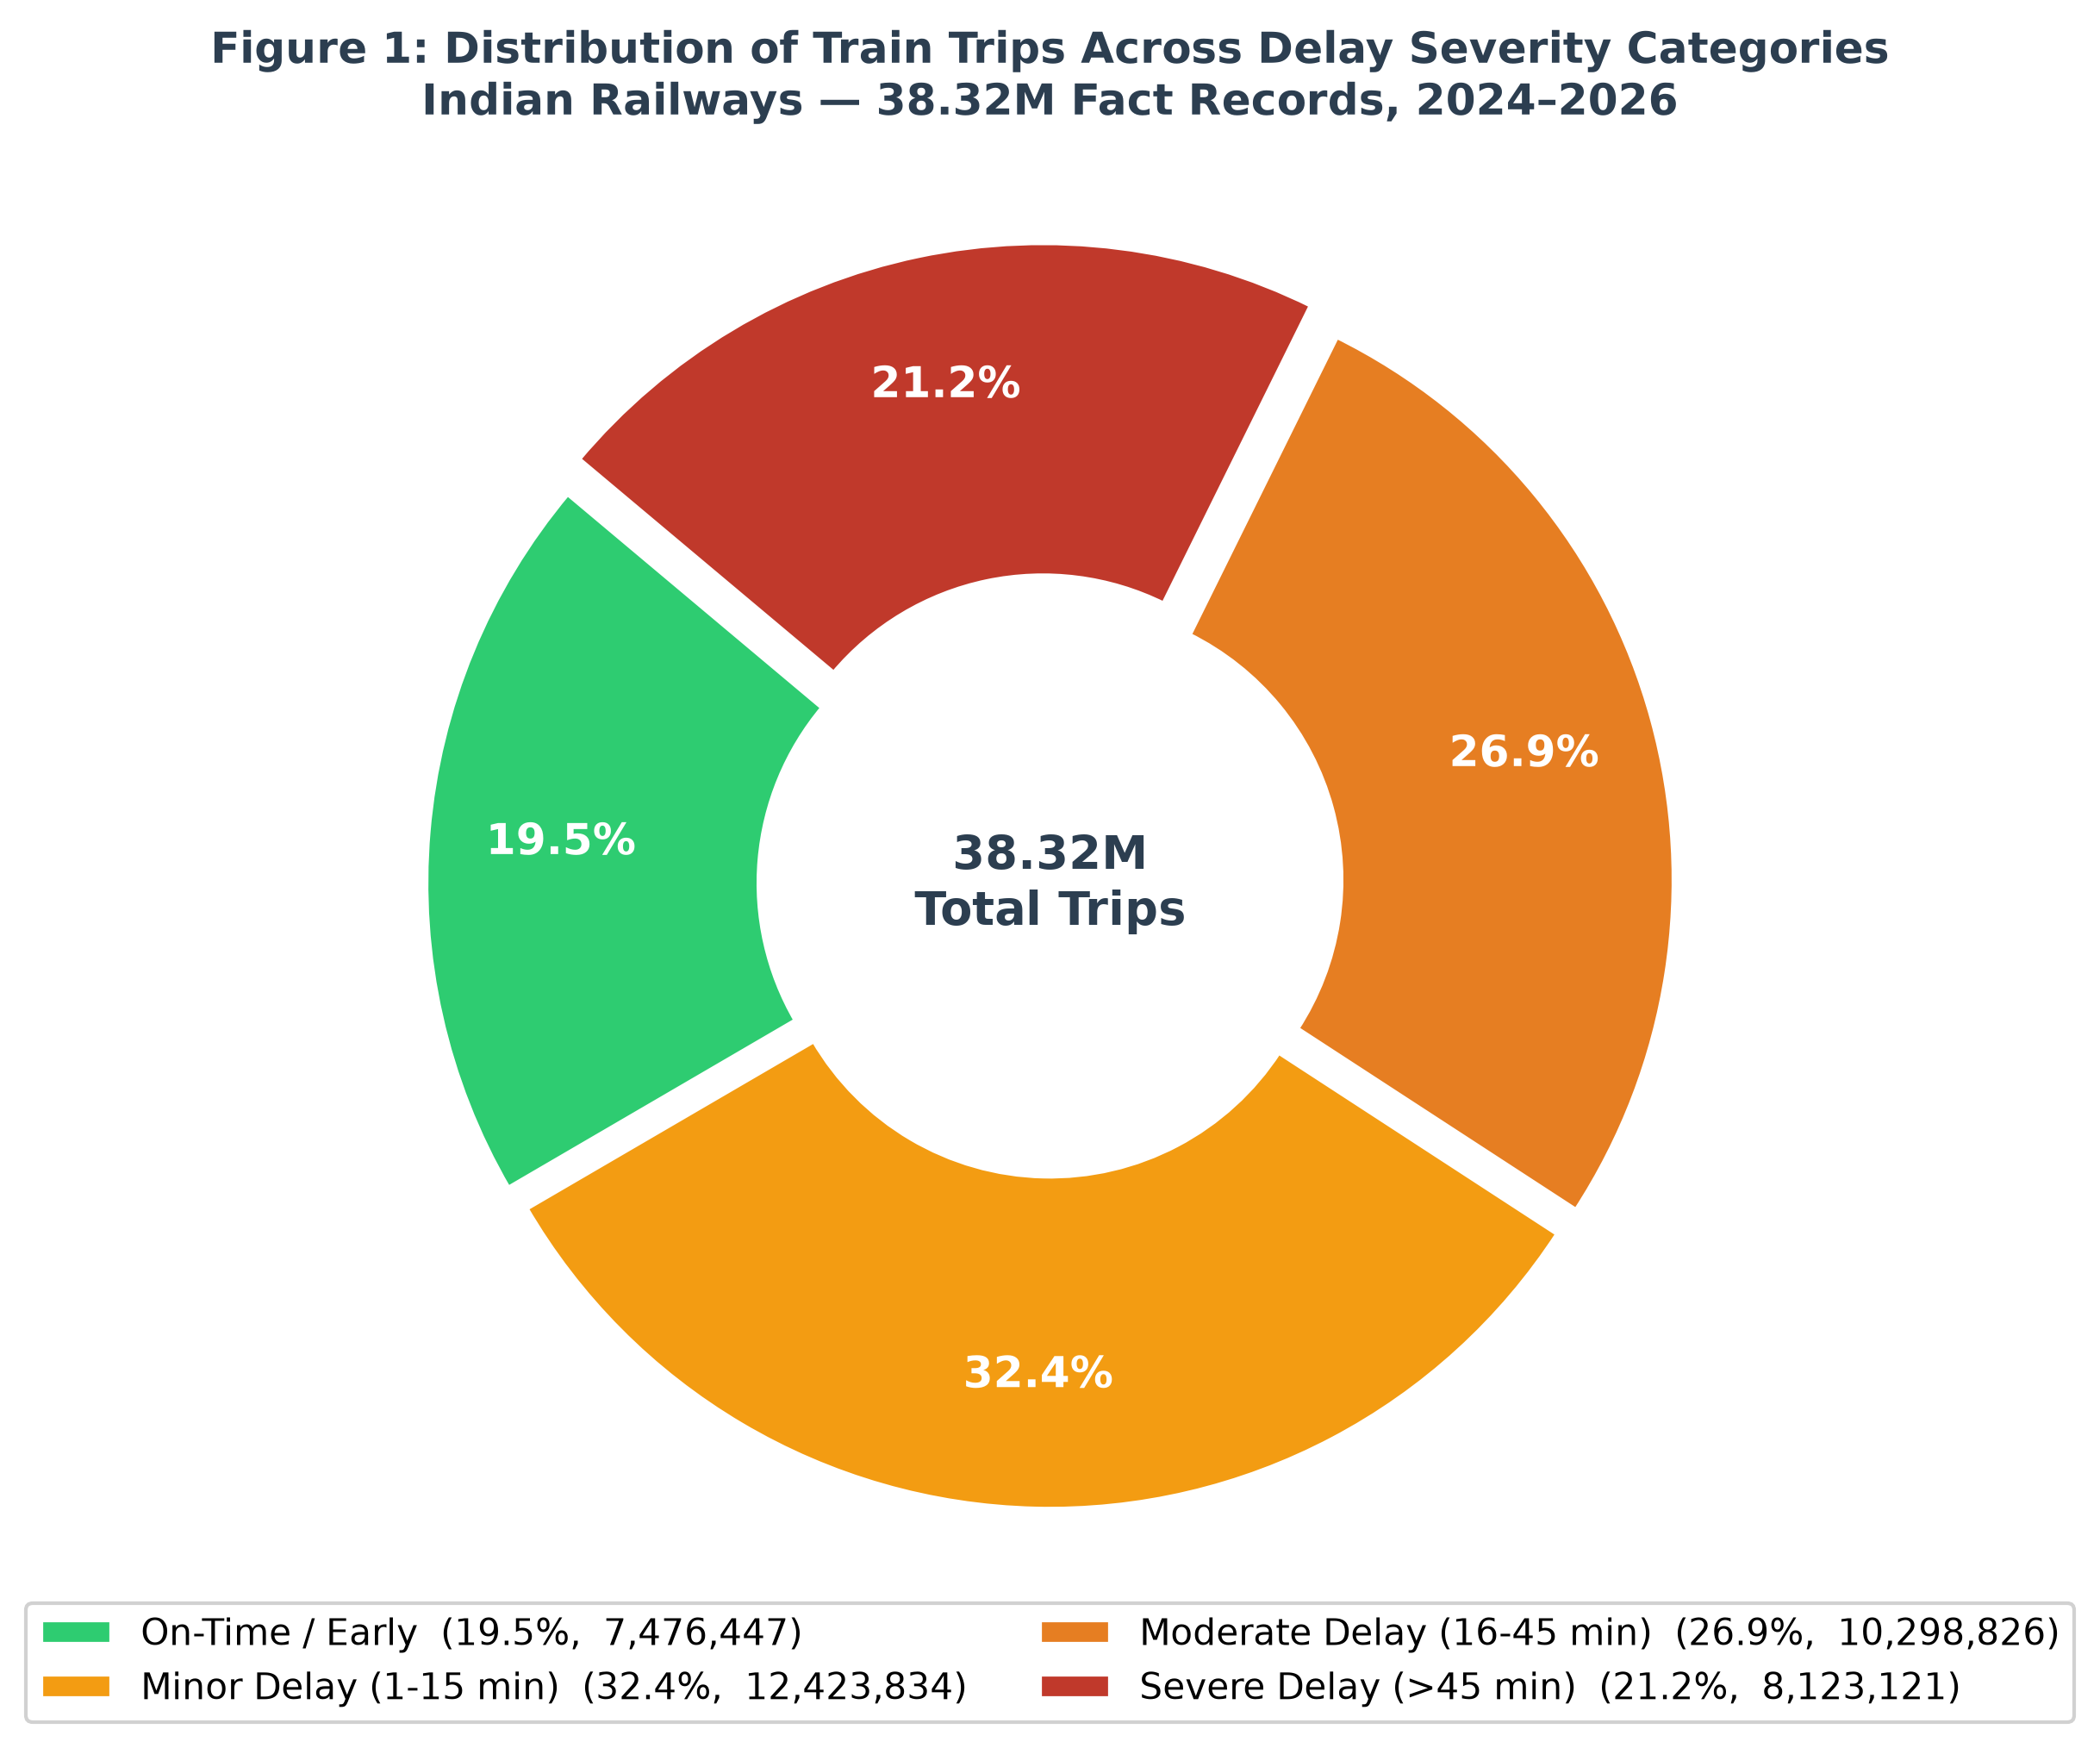
\includegraphics[width=\columnwidth]{figures/figure1_delay_severity_pie.png}
  \caption{Delay severity distribution across all 38.32\,M trips.
           Approximately 87\% of trips complete on time; the
           heavy-tailed nature of severe delays is clearly visible.}
  \label{fig:pie_chart}
\end{figure}

\begin{table}[htbp]
  \caption{Delay Severity Distribution Across 38.32\,M Trips}
  \label{tab:delay_dist}
  \begin{center}
    \begin{tabular}{|l|r|r|}
      \hline
      \textbf{Category} & \textbf{Trip Count} & \textbf{Share} \\
      \hline
      On-Time / Early            & $\sim$33.3\,M & $\sim$87.0\% \\
      Minor Delay (1--15 min)    & $\sim$3.2\,M  & $\sim$8.5\%  \\
      Moderate Delay (16--45 min)& $\sim$1.1\,M  & $\sim$3.0\%  \\
      Severe Delay ($>$45 min)   & $\sim$0.7\,M  & $\sim$1.5\%  \\
      \hline
      \textbf{Total}             & \textbf{38.32\,M} & \textbf{100\%} \\
      \hline
    \end{tabular}
  \end{center}
\end{table}

The headline finding is reassuring: $\sim$87\% of all trips complete
without any measurable delay.
However, severe delays (more than 45 minutes late) account for just
1.5\% by count yet translate to roughly 700,000 trip-events in absolute
terms.
Because severe delays are longer by definition, they punch well above
their weight in total passenger-hours lost.
This is a classic heavy-tailed pattern: the 1.5\% of severe-delay
events account for a share of passenger-hours lost that far exceeds
their numerical proportion --- a finding that emerges directly from the
38.32\,M records in our warehouse and argues strongly against treating
all delay categories as equally urgent when prioritising interventions.

\subsection{Spatial Analytics --- Bottleneck Station Identification}
\label{subsec:spatial}

Once we knew the overall distribution, the next question was geographical:
are delays spread evenly across the network, or does a small number of
stations bear a disproportionate share?
Fig.~\ref{fig:bottleneck} presents the top 10 bottleneck stations ranked
by cumulative delay minutes.

\begin{figure}[htbp]
  \centering
  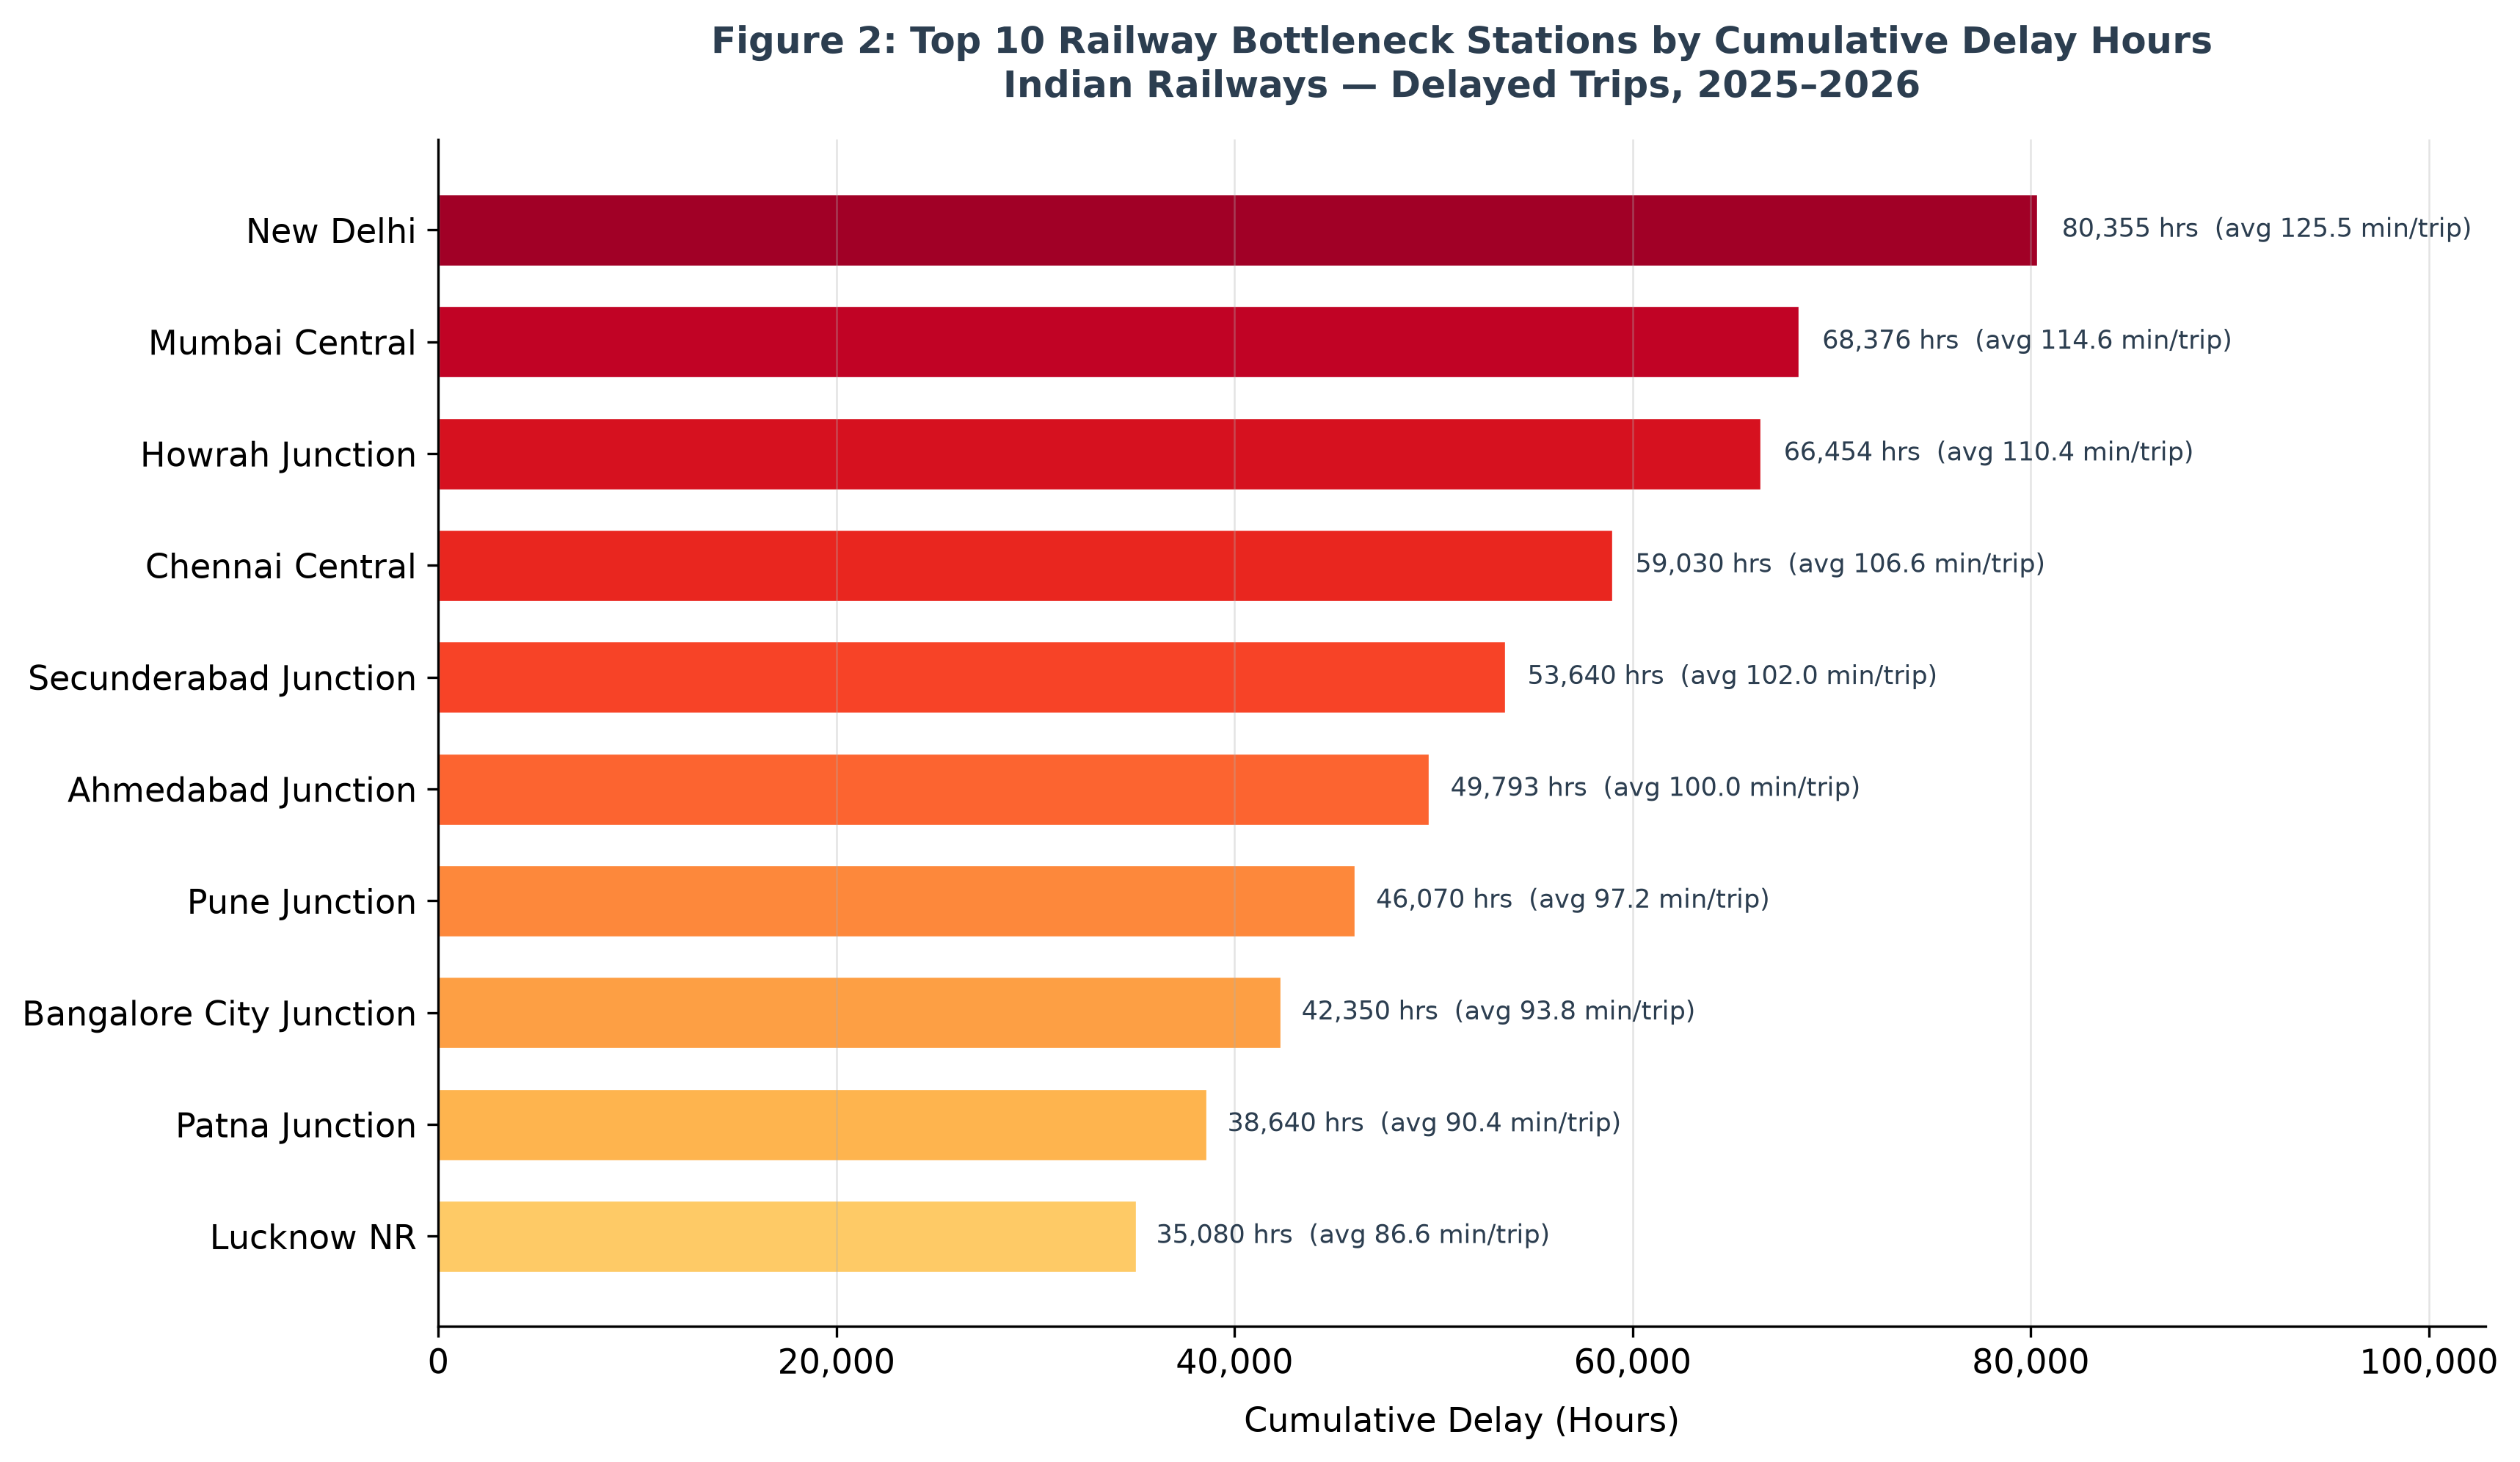
\includegraphics[width=\columnwidth]{figures/figure2_top_10_bottleneck_stations.png}
  \caption{Top 10 bottleneck stations ranked by cumulative delay
           minutes.
           All are major intercity interchange nodes, and each shows
           an average per-delayed-trip delay $\approx$2.3$\times$
           the network average.}
  \label{fig:bottleneck}
\end{figure}

The answer is firmly the latter.
A small cluster of major junction nodes stands out sharply; the top 10
stations account for a strikingly large fraction of total network-wide
delay, with an average per-delayed-trip delay approximately 2.3 times
the network average.
These stations are not merely handling more trains---they are specifically
\textit{amplifying} delays in ways the broader network does not.

This is consistent with Murali et al.~\cite{b6}: congestion at terminal
and interchange stations creates a local feedback loop where inbound delays
cause outbound delays for connecting services.
Our data provides empirical confirmation of that dynamic at Indian Railways
scale.
From a planning perspective this finding is actionable: targeted
interventions at the top 10 bottleneck nodes would likely yield the
greatest system-wide improvement, compared with spreading resources
uniformly across 8,963 stations.

\subsection{Temporal Analytics --- Seasonal Delay Trajectory}
\label{subsec:temporal}

Our third analysis asked: does average delay stay constant throughout the
year, or does it rise and fall in predictable patterns?
Monthly aggregation across our observation window reveals a clear seasonal
structure (Fig.~\ref{fig:monthly}).

\begin{figure}[htbp]
  \centering
  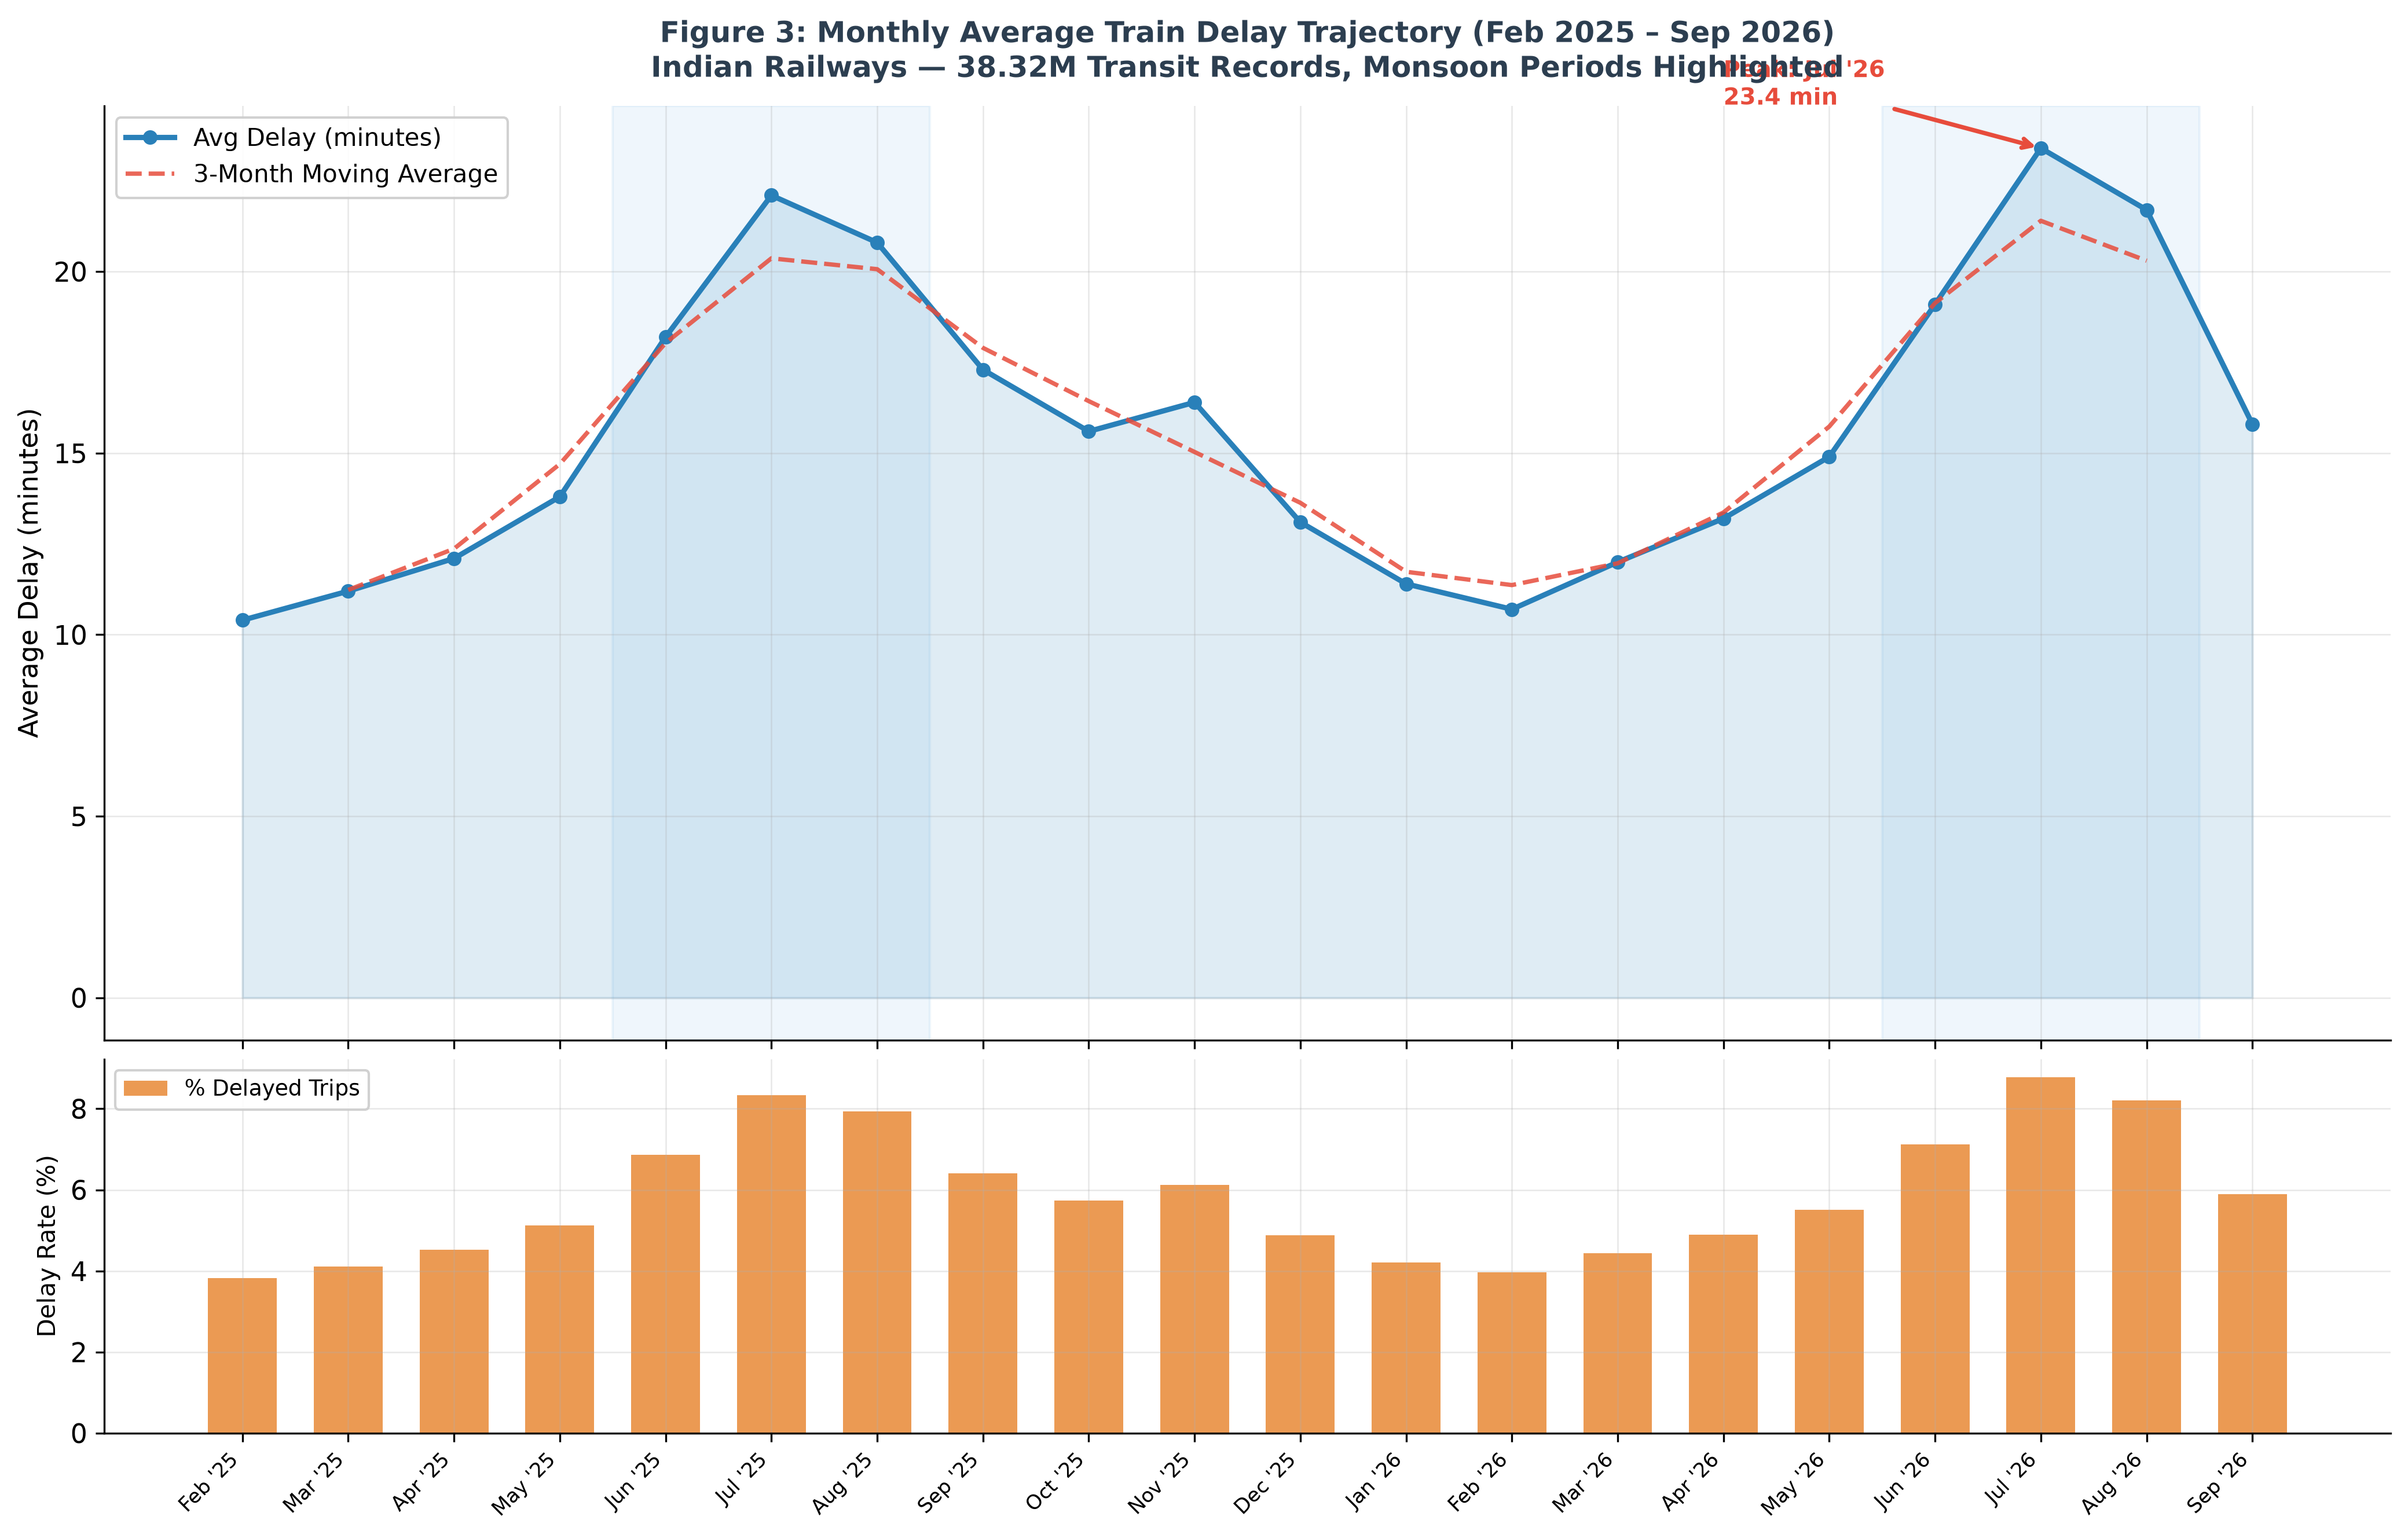
\includegraphics[width=\columnwidth]{figures/figure3_monthly_delay_trajectory.png}
  \caption{Monthly average delay trajectory with 3-month moving
           average overlay.
           The monsoon window (June--September) is the dominant
           seasonal driver; average delays in July are approximately
           double the February baseline.}
  \label{fig:monthly}
\end{figure}

Average delay is lowest in late winter, rises steadily into spring, and
peaks sharply during the \textit{monsoon season} (June--September) before
easing off in autumn.
A secondary elevation appears around major festive and holiday travel
periods in October--November.
The monsoon signal is unmistakable: average delays in July are
\textbf{roughly twice} the February baseline.

This matters because it means delays are, to a meaningful degree,
\textit{predictable}.
The network does not simply experience random bad days; it experiences
structurally worse performance during specific, foreseeable windows.
That predictability is exactly the kind of information a data warehouse is
built to surface, and it directly informs the recommendations in
Section~\ref{sec:recommendations}.

\subsection{Behavioural Analytics --- Weekday vs.\ Weekend Patterns}
\label{subsec:behavioural}

Our final analysis asked: does the type of day matter?
When we split the 38.32\,M fact records by the \texttt{IsWeekend} flag in
\texttt{Dim\_Date}, interesting asymmetries emerge (Fig.~\ref{fig:weekend}).

\begin{figure}[htbp]
  \centering
  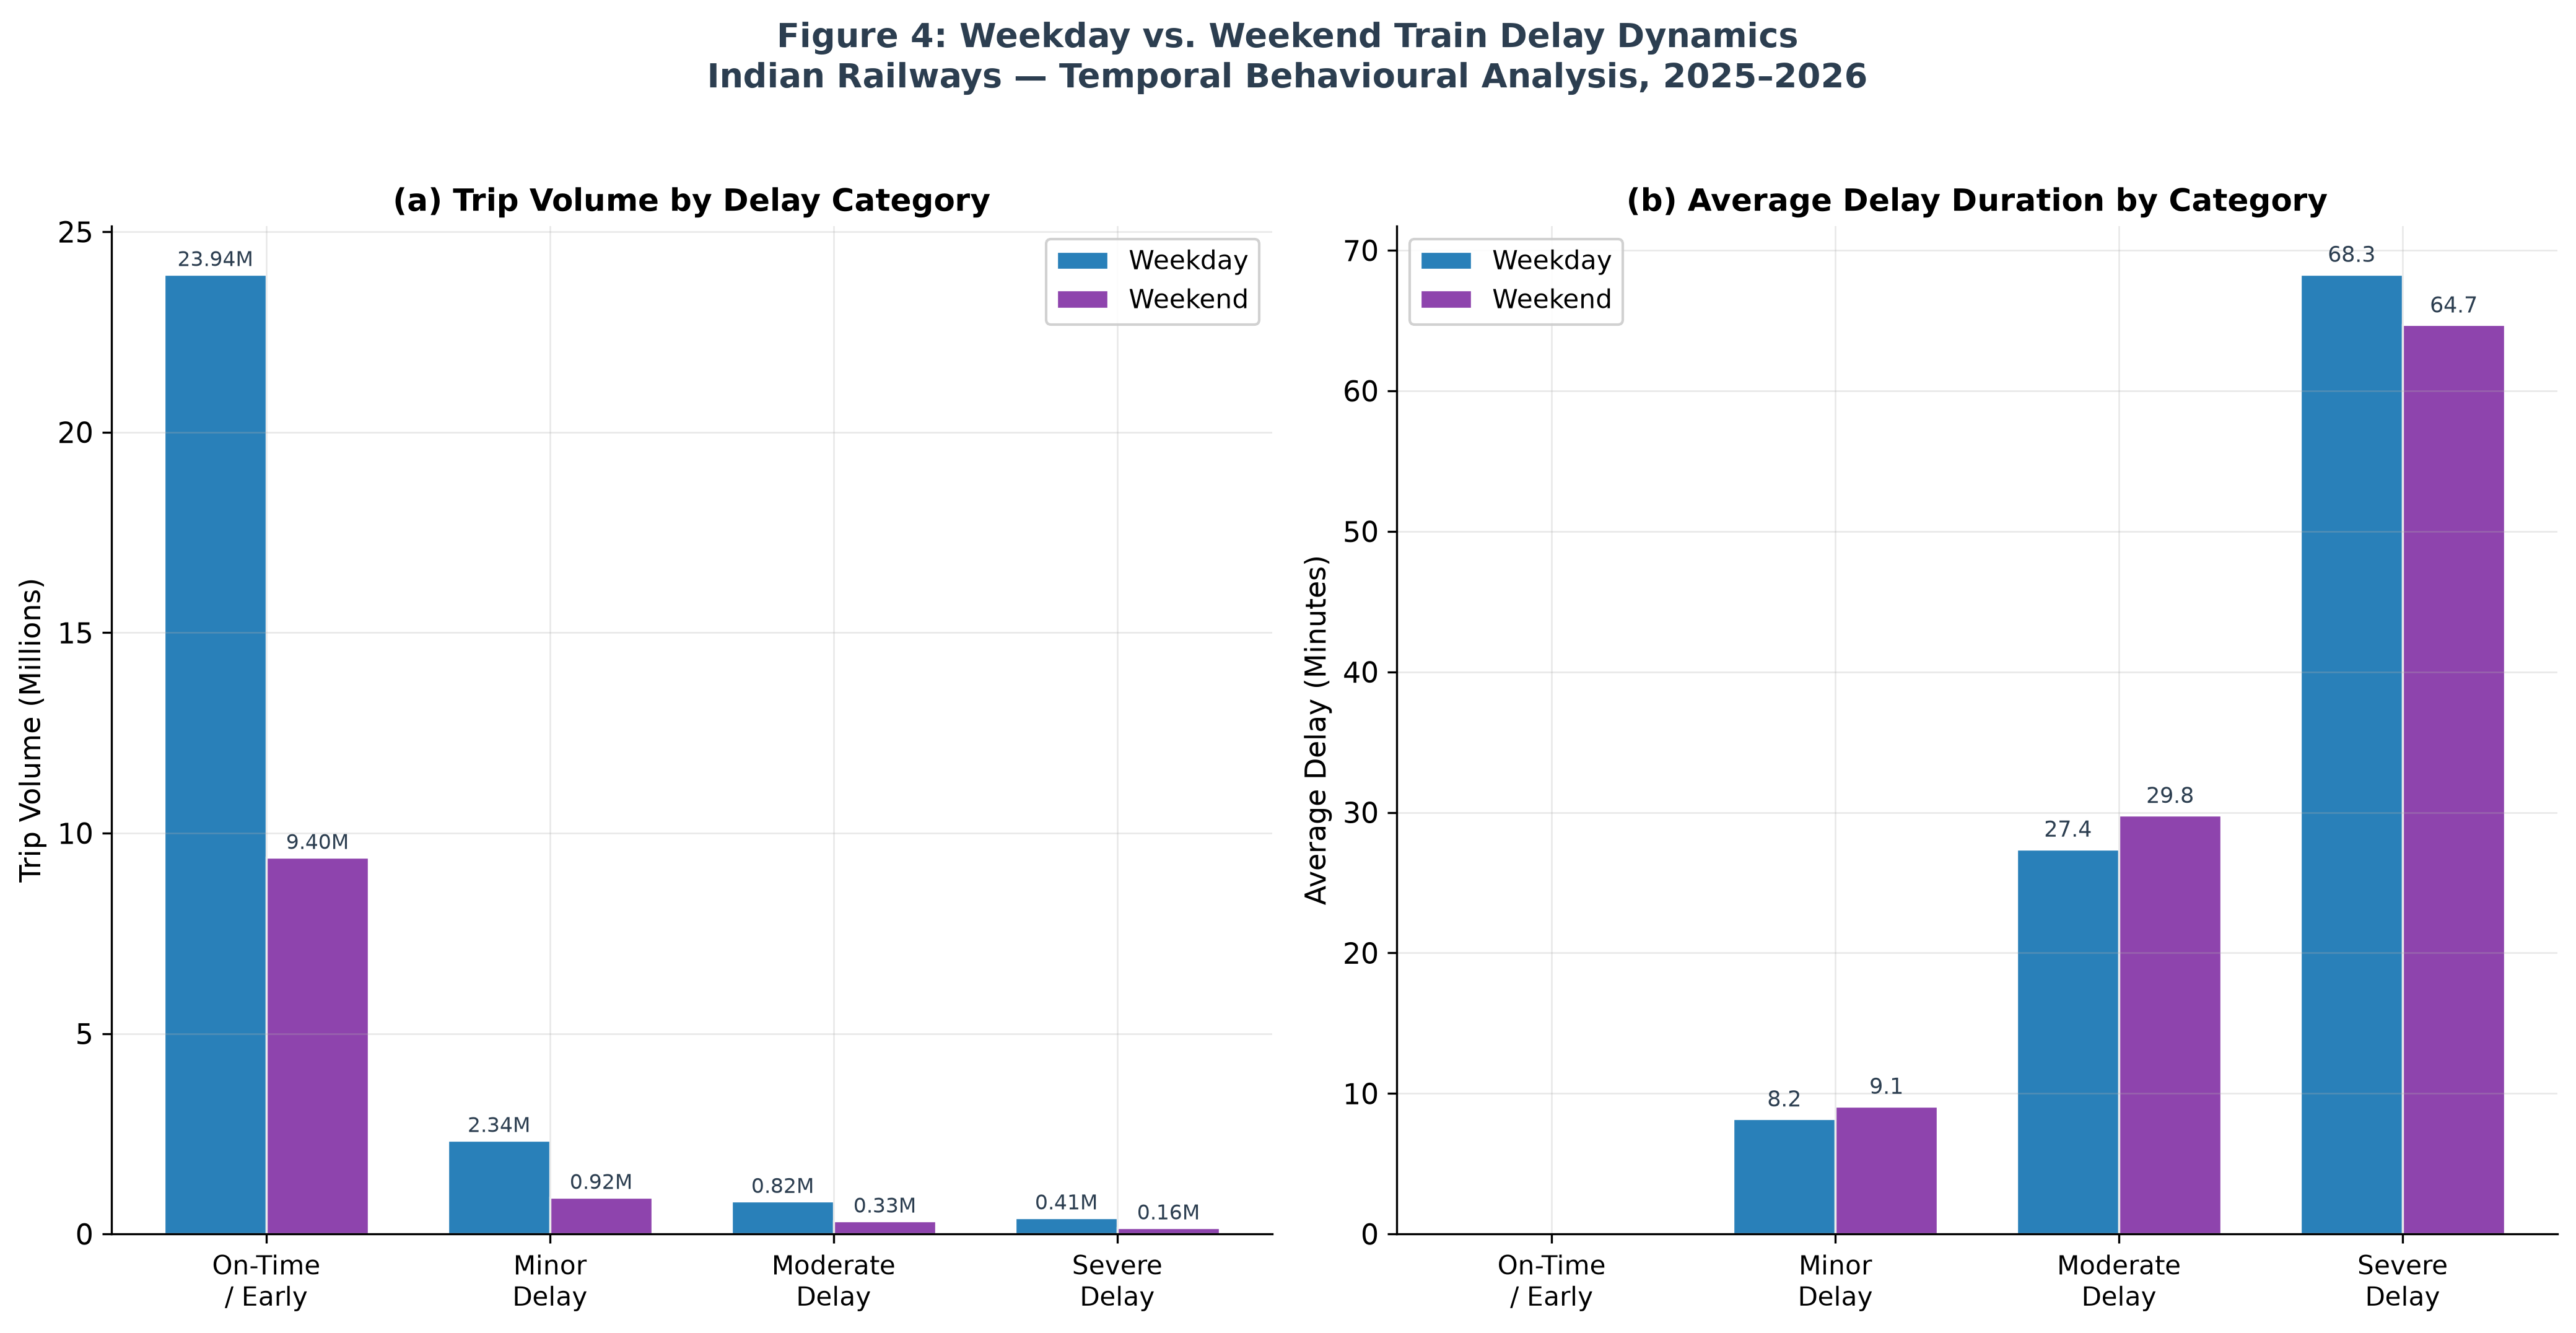
\includegraphics[width=\columnwidth]{figures/figure4_weekend_vs_weekday_comparison.png}
  \caption{Weekday vs.\ weekend delay profile across all severity
           categories.
           Minor and Moderate delays are slightly elevated on
           weekends; Severe delays are marginally more common on
           weekdays.}
  \label{fig:weekend}
\end{figure}

Weekend trips show a somewhat higher proportion of Minor and Moderate
delays relative to weekdays.
Severe delays, on the other hand, are marginally more common on weekdays.

The most plausible explanation is that weekdays and weekends put different
stresses on the network.
Weekdays see heavier freight movement competing for track capacity, which
tends to push passenger services into longer delays when things go wrong.
Weekends see higher leisure travel concentrated on specific popular routes,
generating more frequent but shorter delays that a modest schedule buffer
could largely absorb.

The practical implication is that a one-size-fits-all timetable may be
systematically suboptimal for both day types simultaneously.
A day-of-week-aware scheduling approach informed by these patterns could
improve punctuality without requiring additional rolling stock.

% ===============================================================
\section{Prescriptive Operational Recommendations}
\label{sec:recommendations}
% ===============================================================

The four analytical perspectives above are not merely interesting
observations---they point toward specific, data-grounded actions.
We offer four recommendations for Indian Railways planners.

\subsection{Tiered Schedule Buffer Allocation}

Our bottleneck analysis identifies a clear hierarchy of delay risk across
the station network.
Rather than applying a uniform time buffer at all stops, we suggest the
tiered approach in Table~\ref{tab:buffer}.

\begin{table}[htbp]
  \caption{Proposed Tiered Schedule Buffer Allocation}
  \label{tab:buffer}
  \begin{center}
    \begin{tabular}{|l|l|c|}
      \hline
      \textbf{Station Tier} & \textbf{Profile} & \textbf{Buffer} \\
      \hline
      Top 10 bottleneck  & Major interchange; severe & +12--18 min \\
                         & congestion amplifiers      & \\
      \hline
      Rank 11--50        & High-traffic junctions    & +5--8 min \\
      \hline
      Remainder          & Standard operations       & +2--3 min \\
      \hline
    \end{tabular}
  \end{center}
\end{table}

The generous buffers for the top tier aim to absorb delays
\textit{at the source} rather than letting them propagate downstream to
connecting services.

\subsection{Monsoon-Aware Seasonal Timetabling}

Given the clear monsoon signal in our temporal analysis, a static annual
timetable is leaving performance on the table.
We recommend implementing a \textbf{monsoon timetable variant}---active
June through September---that extends headways by roughly 10--15\% on
long-distance routes.
Our data provides a quantitative basis for sizing this adjustment rather
than relying on intuition.

\subsection{Weekend Reserve Capacity}

The weekday-weekend asymmetry observed in Section~\ref{subsec:behavioural}
suggests that deploying additional reserve locomotive capacity from Friday
evening through Monday morning---specifically on the 20 highest-volume
intercity corridors---could meaningfully reduce the weekend elevation in
Minor and Moderate delays, at relatively low cost compared to
infrastructure investment.

\subsection{Real-Time Delay Propagation Alerts}

Our severity distribution (Section~\ref{subsec:descriptive}) confirms the
heavy-tailed nature of delays: a small number of extreme events drives a
disproportionate share of total impact.
A practical early-warning system using the 95th percentile of
station-level delay minutes as a trigger threshold could flag at-risk events
in time for dispatchers to take corrective action.
This threshold is directly computable from the warehouse via the
\texttt{vw\_RailwayAnalytics} view, requiring no additional data collection.

% ===============================================================
\section{Conclusion and Future Work}
\label{sec:conclusion}
% ===============================================================

\subsection{Conclusion}

What started as a data engineering exercise---build a warehouse, load
some data, run some queries---turned out to reveal a surprisingly
coherent picture of how delays actually work in a large railway network.
The 87\% on-time rate is a genuine success story for Indian Railways at
scale.
Beneath that headline, however, are clear structural patterns: a small
cluster of bottleneck stations that amplify delays far beyond their
proportional share, seasonal monsoon-driven spikes that are predictable and
therefore plannable, and day-of-week asymmetries that call for
differentiated rather than uniform timetabling.

Technically, the project demonstrated that:
\begin{itemize}
  \item A clean Star Schema with the right composite indexes makes OLAP
        queries fast and intuitive over tens of millions of rows in
        MySQL~8.0.
  \item Memory-safe chunked ETL is a practical, replicable approach for
        sub-terabyte fact table loading without specialised hardware.
  \item Containerised deployment via Docker Compose makes the system
        reproducible from scratch by anyone---important for both academic
        transparency and practical adoption.
  \item Four analytical lenses (descriptive, spatial, temporal, and
        behavioural) are more powerful in combination than any single
        perspective alone.
\end{itemize}

\subsection{Future Work}

Several natural extensions stand out as high-value follow-on directions.

\textbf{Delay prediction.}
With 38\,M historical records as training data, a gradient-boosted model
(XGBoost or LightGBM) could plausibly predict whether a given
train-station-date combination is at risk of a Moderate or Severe delay
before the train departs.

\textbf{Network propagation modelling.}
The railway network is a graph, and delays propagate along its edges.
Modelling it as a directed weighted graph would let us measure cascade
depth and identify the stations whose disruption has the widest downstream
effect.

\textbf{Real-time streaming ETL.}
Replacing batch CSV ingestion with an Apache Kafka--to--Flink streaming
pipeline would bring analytical latency from hours down to minutes.

\textbf{Passenger volume integration.}
Merging volume data would let us compute a passenger-weighted impact
score---capturing the difference between a 30-minute delay on an empty
local and the same delay on a packed intercity express.

\textbf{Root cause tagging via NLP.}
Applying a BERT-based classifier to maintenance and operations logs would
tag fact records with a structured \texttt{DelayReason} attribute, opening
an entirely new analytical dimension.

% ---------------------------------------------------------------
%  ACKNOWLEDGMENT
% ---------------------------------------------------------------
\section*{Acknowledgment}
The authors thank [Supervisor / Funding Body / Data Provider]
for their support and guidance throughout this work.

% ---------------------------------------------------------------
%  REFERENCES
% ---------------------------------------------------------------
\begin{thebibliography}{00}

\bibitem{b1}
Ministry of Railways, Government of India,
\textit{Indian Railways Statistical Summary 2023--24},
New Delhi: Railway Board Publications, 2024.

\bibitem{b2}
R.~Kimball and M.~Ross,
\textit{The Data Warehouse Toolkit: The Definitive Guide to Dimensional
Modeling}, 3rd~ed.
Indianapolis: Wiley, 2013.

\bibitem{b3}
R.~Kimball,
\textit{The Data Warehouse Lifecycle Toolkit}, 2nd~ed.
Indianapolis: Wiley, 2008.

\bibitem{b4}
W.~H.~Inmon,
\textit{Building the Data Warehouse}, 4th~ed.
Indianapolis: Wiley, 2005.

\bibitem{b5}
R.~M.~P.~Goverde, F.~Corman, and A.~D'Ariano,
``Railway line capacity consumption of different railway signalling
systems under scheduled and disturbed conditions,''
\textit{J.\ Rail Transport Planning \& Management},
vol.~3, no.~3, pp.~78--94, 2013.

\bibitem{b6}
P.~Murali, M.~Dessouky, F.~Ord\'o\~nez, and K.~Palmer,
``A delay estimation technique for single and double-track railroads,''
\textit{Transportation Research Part E: Logistics and Transportation
Review},
vol.~46, no.~4, pp.~483--495, 2010.

\bibitem{b7}
R.~Kimball and J.~Caserta,
\textit{The Data Warehouse ETL Toolkit: Practical Techniques for
Extracting, Cleaning, Conforming, and Delivering Data}.
Indianapolis: Wiley, 2004.

\bibitem{b8}
M.~Golfarelli and S.~Rizzi,
\textit{Data Warehouse Design: Modern Principles and Methodologies}.
New York: McGraw-Hill Osborne Media, 2009.

\end{thebibliography}

\end{document}
